\documentclass[main.tex]{subfiles}
\begin{document}

\chapter{Results}

\section{The Data Sets}
The data presented in this chapter was collected during one hour of parallel measurements with both the analog and the digital setup. A total of 4.3 million pulses from the NE213 detector were recorded by the analog setup, while the digitizer only saw 2.2 million pulses after the selection criteria explained in the previous chapter were applied. This large difference in count rates is because the digital setup was configured to transfer each event individually. Furthermore the software WaveDump does not have a method for estimating livetime, so instead a livetime will be estimated by comparing with the analog setup.

Thresholds of 25.0 mV and 94.6 mV were applied to the YAP and the NE213 detector respectively in the analog setup, while the digital setup applied thresholds of 9.8 mV and 48.8 mV on the YAP and the NE213 detector. Having such a low threshold on the YAP was found to decrease the signal to noise ratio in the time of flight spectrum, so a higher threshold of 24.4\si{\milli\volt} was applied in software.
\begin{table}[bh]
\begin{tabular}{|l|l|l|l|l|}
\hline
Setup   & YAP threshold(mV) & NE213 threshold(mV) & NE213 events ($\text{10}^\text{6}$) & Livetime \\ \hline
Analog  & 25.0              & 94.6                & 4.3      & 44\%             \\ \hline
Digital & 9.8/24.4*			& 48.8                & 2.2      & **             \\ \hline
\end{tabular}
\caption{Overview table of the two data sets. *The higher threshold was enforced offline (see text for details). **The digital setup does not have a method for determining livetime}
\label{tab:settings}
\end{table}

\section{The Analog Setup}

\subsection{Neutron Tagging}
Figure \ref{fig:tof_a} shows the time of flight spectrum recorded by the analog setup. The neutron and gamma ray peaks marked with arrows. In addition to these two peaks there is an approximately flat background. This background represent uncorelated particles triggering start and stop, which is why negative time of flight values appear.
\begin{figure}[ht]
    \centering
        \includegraphics{AnalogResults/tof.pdf}
        \caption{The time of flight spectrum. The x-axis denotes the time of flight from source to NE213 detector. The neutron and gamma peaks have been indicated with arrows. The coincidences highlighted in red have been converted to neutron kinetic energies and are shown in the upper right insert.}
    \label{fig:tof_a}
\end{figure}

The gamma ray peak has been shifted to be centered at \SI{3.5}{ns}, but it is not entirely narrow. Since the gamma rays travel at the speed of light one might expect a much narrower gamma peak. This is primarily due to the time resolution of the detector as well as attenuation in the cables, which might affect pulse shape and thus rise time. This will in turn make the constant fraction discriminator less effective causing some loss in the time resolution. Furthermore, the final  digitization by the TDCs may cause some loss of resolution. Differences in flight path between gammas hitting the center of the NE213 and those that hit near the edge will be less than 1 cm, so this will not give rise to a substantial time spread. 

The neutron peak has faster neutrons at lower time of flight values and slower neutrons at higher time of flight values. Since the distance from source to detector is known it is possible to convert the neutron time of flight into kinetic energy. A range of 1.5-\SI{7}{\MeV} was converted to a time interval of 29-\SI{62}{\ns}. The coincidences falling in this time interval have been highlighted in red and the corresponding energies are shown in figure \ref{fig:tof_a}, where higher flight times map to lower energies.

Comparing to the spectrum obtained by Scherzinger\cite{ScherzingerPhd} and shown in \ref{fig:scherzinger} a couple of differences stand out. Scherzingers spectrum had peaks around \SI{3}{\MeV} and \SI{4.8}{\MeV}, whereas this spectrum only has a peak at \SI{4.5}{\MeV}. This spectrum on the other hand appears to have a peak near \SI{3.8}{\MeV} and one between 4 and \SI{5}{\MeV}. The absence of the \SI{3}{\MeV} peak may indicate that a higher threshold was applied when acquiring this dataset. At low energies the counts in figure \ref{fig:tof_a} increases. This is simply an effect of the last \SI{10}{\ns} primarily consisting of background, and that the lowest energies covers a wider range of flight time since $E\propto \dfrac{1}{ToF^2}$. beyond \SI{6}{\MeV} the spectrum goes to zero just as seen in the reference spectrum.



\subsection{Pulse Shape Discrimination}
Neutrons and gamma rays were discriminated through the pulse shape parameter given in equation \ref{eq:ps}. The parameters a=120 and b=0 were found to linearize pulseshape as a function of energy, and gate lengths of \SI{500}{\ns} and \SI{60}{ns} were used for the longgate and shortgate integrations respectively.

\begin{figure}[ht]
    \centering
        \includegraphics{AnalogResults/psd.pdf}
        \caption{The pulse shape spectrum as a function of energy deposition. The dashed white line at 0.259 indicates the discrimination cut.}
        \label{fig:psd_a}
\end{figure}

PS is shown as a function of deposited energy in figure \ref{fig:psd_a}. The upper band is made up of pulses for which the tail contained a large fraction of the total charge. This is the neutron band. Conversely The lower band is made up of gamma rays for which a smaller amount of the energy is carried in the tail of the pulse. That this is indeed the case is confirmed by the presence of the \SI{2.23}{MeV} and \SI{4.44}{MeV} gamma ray peaks in the lower band. The amplitude threshold of \SI{94.6}{mV} gives rise to the sloping energy threshold in the figure. This is because pulses with higher PS parameter (more charge in tail) will contain more total charge than a pulse of equal amplitude but smaller PS parameter.


events below 0.8 MeV are mostly the result of the pedestal injection, and consequently they are not of interest for pulse shape discrimination and have been removed.

The linearization made it possible to separate the neutron and gamma ray bands at a single PS value. The procedure by which this cut was determined will be presented in section \ref{sec:comp}. For now it will just be noted that PS=0.259, shown as a dashed line in figure \ref{fig:psd_a}, was found to provide the best separation. Seeing how the neutron and gamma ray distributions seem to overlap at low energies this cut will likely result in misclassification. The time of flight information provides an independent parameter for distinguishing the particle species and can therefore be used to quantify the extent of the misclassification.

Figure \ref{fig:tof_ps_a} shows pulse shape as a function of time of flight, with neutron and gamma distributions highlighted. The gamma ray and neutron distributions, marked with arrows, are somewhat overlapping, making the discrimination cut mislabel part of each distribution.

Often the start and stop signal will be due to uncorrelated particles, rather than the previously discussed n-\textgamma and \textgamma-\textgamma pairs. On small timescales of a few hundred nanoseconds these events are expected to form a flat background in the time of flight spectrum, as seen in figure \ref{fig:tof_a} beyond 60 ns. Since the events still represent either neutrons or gamma rays (ignoring the occasional muon) one would expect them to be separated into two bands in figure \ref{fig:tof_ps_a}. This is not the case.

Another interesting feature is that there is large amount of gamma rays at higher PS values. This is because not all the events produced by the pedestal injection were removed by the cut at 0.8 $\text{MeV}_\text{ee}$ and as these events use the same signal as start and stop, they will appear near the gamma peak. The reason why they have such a high fraction of PS lies in the gate lengths. Since the charge integrals of these events are just integrals of what randomly happened to be in the detector at the time a YAP trigger occured, and since the longgate window is more than eight time as long as the shortgate window it is more likely that there is something to integrate in the tail part of the window.






\begin{figure}[ht]
    \centering
        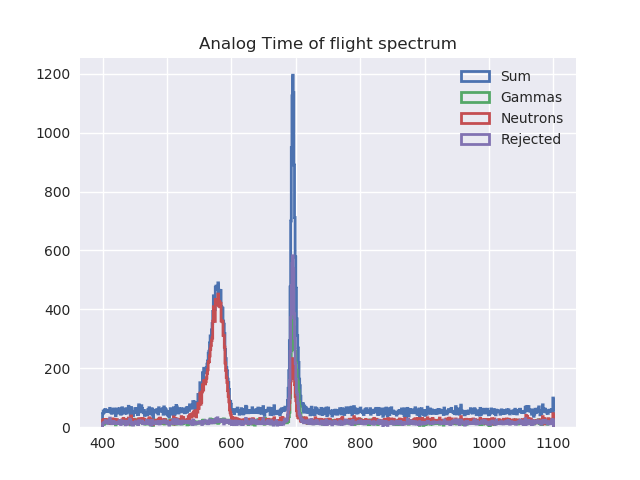
\includegraphics{AnalogResults/tof_psd.pdf}
        \caption{Time of flight plotted against pulse shape as recorded with the analog setup. The dashed white line indicates the discrimination cut at PS=0.259. A logarithmic z-axis is used to highlight the distribution of background events.}
    \label{fig:tof_ps_a} 
\end{figure}



%We can gain some more information on the effect of the injected pedestal events by looking at figure \ref{fig:tof_E_a}. Above 0.8 $\text{MeV}_\text{ee}$ We have a gamma and a neutron distribution as marked by the arrows. It is also clear that the events produced by triggering on YAP signals (less than 0.8 MeV) mostly land near the gamma ray time of flight. This is to be expected since these signals are acting as both start and stop signals. It is also clear that the cut at 0.8 $\text{MeV}_\text{ee}$ will not be able to remove all of these events. Unlike the gamma flash the neutron distribution show some correlation between time of flight and energy deposition. It seems that the faster neutrons are able to deposit more energy than the slower ones.
%
%In figure \ref{fig:tof_Edep_Eneutron_a} the deposited energy is shown as a function of neutron kinetic energy as found from the time of flight spectrum. It can be seen that high energy deposition implies high neutron energy. However, the converse is not necessarily true as neutrons may scatter out of the detector before depositing all their energy. It is interesting that the energy the detector sees in $\text{MeV}_\text{ee}$ appears to be only half of the neutrons kinetic energy in  $MeV$.
%
%\begin{figure}[ht]
%    \centering
%        \includegraphics{AnalogResults/tof_E.pdf}
%        \caption{Time of flight plotted against energy deposition.}
%    \label{fig:tof_E_a} 
%\end{figure}
%
%\begin{figure}[ht]
%    \centering
%        \includegraphics{AnalogResults/tof_Edep_Eneutron.pdf}
%        \caption{Neutron energy as a function of deposited energy in the NE213 detector.}
%    \label{fig:tof_Edep_Eneutron_a} 
%\end{figure}
%
%





\section{Digital setup}

\subsection{Neutron Tagging}
The time of flight spectrum acquired in the 1 hour of data taking is shown in figure \ref{fig:tof_d}. The gamma and netron peaks are indicated with arrows. The gamma peak is not entirely narrow as one might expect seeing as they all travel at the speed of light. The main reason for this is the intrinsic time resolution of the detector and as well as the digitization of the pulse. The CFD algorithm looks for where the pulse crosses 30\% of maximum amplitude, but the determination of the maximum amplitude is limited by the resolution and sampling rate of the digitizer.

The flight times in the neutron peak, marked with dotted red lines, has been used to generate the energy spectrum shown in the upper right insert of figure \ref{fig:tof_d}. The spectrum goes to lower energies than what we see for the analog setup in figure \ref{fig:tof_a}, this may be because the digital setup has a lower amplitude threshold than the analog setup, allowing slower neutrons to be recorded.
\begin{figure}[ht]
    \centering
        \includegraphics{DigitalResults/tof.pdf}
        \caption{The time of flight spectrum of the PuBe source produced by the digital setup.}
    \label{fig:tof_d} 
\end{figure}



\subsection{Pulse shape discrimination}
Just like with the analog setup the charge integrals were used to perform pulse shape discrimination. The resulting PSD heatmap is shown figure \ref{fig:psd_d}. Since a lower amplitude threshold was applied to the digital setup we find a lot of low energy gamma rays in the gamma band. The 2.23 $MeV_{ee}$ and 4.44 $MeV_{ee}$ compton edges are also clearly distinguishable. 

As with the analog setup longgate and shortgate offsets can be used to linearize the seperation between the bands. Here each shortgate sample point has been offset by 4.79 mV while each longgate sample has been offset by 0.24 mV. At lower energies the bands intersect, but above 1.5 MeV they are clearly separated.

\begin{figure}[ht]
    \centering
        \includegraphics{DigitalResults/psd.pdf}
        \caption{Pulse shape discrimination spectrum produced with the charge comparisson method.}
        \label{fig:psd_d}
\end{figure}

%\subsection{Convolutional Neural Network}
The convolutional neural network described in \ref{sec:cnn} was applied to the digitized waveforms. Since the activation function of the output node is the logistic function the value is bounded between zero and one. The resulting pulse shape discrimination spectrum is shown in figure \ref{fig:cnn_E} as a function of deposited energy. Like for the charge comparisson method the upper distribution is neutrons and the lower distribution consists of gamma rays. The bands are better separated here than by the charge comparison method although there still is some slight overlap at low energies. Again the 2.23 and 4.44 $MeV_{ee}$ Compton edges are clearly visible in the gamma band. 

\begin{figure}[ht]
    \centering
        \includegraphics{DigitalResults/CNNpsd.pdf}
        \caption{Pulse shape discrimination spectrum produced with a convolutional neural network.}
    \label{fig:cnn_E} 
\end{figure}

In order to test the two pulse shape discrimination algorithms one can plot their pulse shape parameters against time of flight. This is shown in figure \ref{fig:tof_cc_tof_cnn}. Figure \ref{fig:tof_digi_cc} shows the narrow gamma distribution and the wider neutron distribution as separated by the charge comparisson method. It is apparent that the two distributons overlap somewhat in pulse shape. It is of note that the neutron and gamma background forms two slightly separated bands.  In figure \ref{fig:tof_digi_cnn} it can be seen that the CNN method provides a better separation, although it still appears that gamma and neutron distributions overlap slightly near prediction value 0.5. The distribution of random coincidence events clearly separate into a gamma ray band below the cut and a neutron band above it.


\begin{figure}
    \centering
    \begin{subfigure}[ht]{\textwidth}
        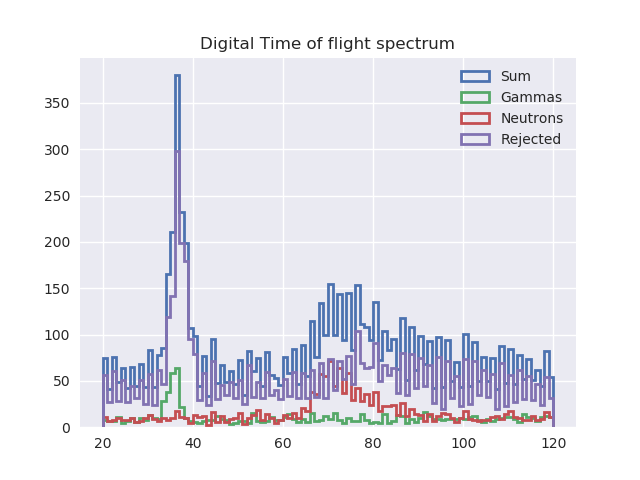
\includegraphics{DigitalResults/tof_psd.pdf}
        \caption{}
        \label{fig:tof_digi_cc}
    \end{subfigure}
	\begin{subfigure}[ht]{\textwidth}
        \includegraphics{DigitalResults/CNNtof_psd.pdf}
        \caption{}
        \label{fig:tof_digi_cnn}
    \end{subfigure}
    \caption{Heatmaps of of pulseshape discrimination parameters as functions of time of flight plotted with logarithmic z-axis.}
    \label{fig:tof_cc_tof_cnn}
\end{figure}

The heatmap shown in figure \ref{fig:tof_E_d} shows energy deposition in the NE213 detector as a function of time of flight. This spectrum hints at why the gamma ray time of flight peak is not entirely narrow. It seems that low energy gamma rays are a bit more spread out regarding time of flight. This could mean that gamma rays traveling at an angle (and thus travelling a slightly longer path) have a higher probability of hitting the detector closer to the edge and get scattered before depositing all of their energy. It could also indicate that the CFD algorithm has a harder time timestamping low charge pulses.

The neutron distribution clearly shows a relation between time of flight and deposited energy. In figure \ref{fig:tof_Edep_Eneutron_d} this relation is highlighted. There appears to be a roughly linear relation between maximum deposited energy and neutron kinetic energy (which determines time of flight). However, as for the analog setup a neutron may deposit all or only part of its energy, so for a given deposited energy we can only conclude the minimum amount of energy the neutron must have had.


\begin{figure}[ht]
    \centering
        \includegraphics{DigitalResults/tof_E.pdf}
        \caption{Time of flight plotted against energy deposition.}
    \label{fig:tof_E_d} 
\end{figure}

%\begin{figure}[ht]
%    \centering
%        \includegraphics{DigitalResults/%tof_Edep_Eneutron.pdf}
%        \caption{Neutron energy as a function of %deposited energy in the NE213 detector.}
%    \label{fig:tof_Edep_Eneutron_d} 
%\end{figure}




\begin{figure}[ht]
    \centering
        \includegraphics{DigitalResults/N_E.pdf}
        \caption{Top: Ratio of deposited energy to neutron kinetic energy. Bottom: deposited energy as a function of neutron kinetic energy, along with fits.}
    \label{fig:N_E} 
\end{figure}
\clearpage
\section{Results and Performance Comparisson}\label{sec:comp}
\subsection{Energy Spectra and Livetime}

The analog and the digital setup were run with different amplitude thresholds, so in order to properly compare them the correct threshold need to be found. Since the two setups have different cable lengths to the detectors they are not attenuated to the same extent, so the digital setup will need a significantly higher threshold than the analog setup in order to accept the same events. Figure \ref{fig:qdc_comp} top panel shows the energy and time of flight spectra. It is clear from the energy spectrum that the digital setup has a lower threshold applied In addition to this the analog setup reaches the limit of the QDCs range slightly above \SI{6}{\MeV}$_\text{ee}$, whereas the digital spectrum continues. 

\begin{figure}[h]
    \centering
        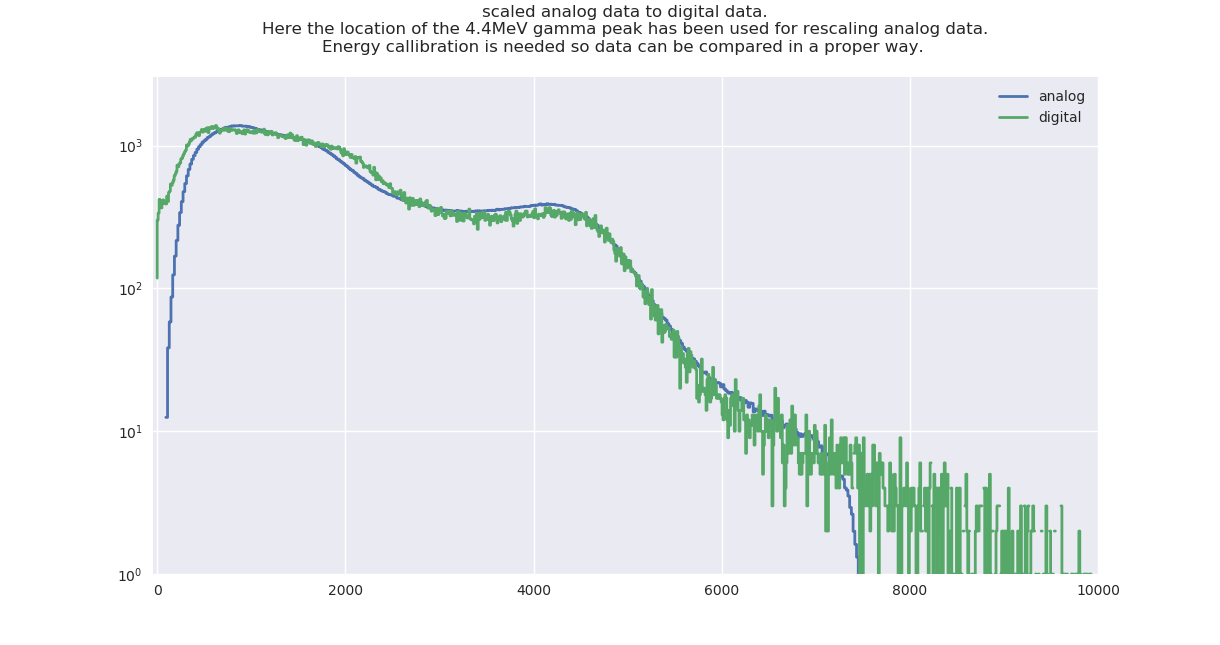
\includegraphics[width=0.8\textwidth]{CompareResults/qdc_comp.pdf}
        \caption{Comparison of analog and digital time of flight spectra. In the lower panel livetime has been taken into account and the digitized data has had a higher threshold enforced on the NE213 signals.}
    \label{fig:qdc_comp}
\end{figure}

In the bottom panel of the figure the threshold has been adjusted to match the analog setup and the counts of the analog setup have been rescaled to compensate for 56\% deadtime. The data acquisition software WaveDump does not offer a way to calculate deadtime\footnote{Although it is possible to make custom software that does this using CAENs libraries}, so instead the digitized data has been scaled to match the data from the analog daq. By carrying out these changes the two energy spectra look more alike, although the \SI{4.44}{\MeV}$_\text{ee}$ Compton edges look quite different. This may be because some of the high energy gamma rays were outside of the dynamic range of the digitizer.

Figure \ref{fig:qdc_ratio} shows the ratio between the digital and analog Energy spectra from after livetime adjustments and threshold alignment. Below \SI{0.8}{\MeV}$_\text{ee}$ the analog setup will pull the ration down due to the pedestal injection and above \SI{6}{\MeV}$_\text{ee}$ the ratio blows up because this is outside the range of the analog QDC modules. Ideally however everything inbetween 0.8 and \SI{6}{\MeV}$_\text{ee}$ should be very close to 1. Initially this seems to be the case, but near the \SI{4.44}{\MeV}$_\text{ee}$ compton edge there is a bump followed by a vally. This is likely because the highest amplitude digitized pulses were clipped, causing them to be pushed to lower values of deposited energy.
\begin{figure}[h]
    \centering
        \includegraphics[width=0.8\textwidth]{CompareResults/QDC_ratio.pdf}
        \caption{Ratio of the digital and analog QDC spectra.}
    \label{fig:qdc_ratio}
\end{figure}

\subsection{Time of Flight Spectra}
Like the energy spectrum the time of flight is heavily influenced by the choice of amplitude threshold. Figure \ref{fig:tof_comp} top panel shows the time of flight spectra for the two setups with the intial 49 mV NE213 threshold on the digital setup and 94.6 mV on the analog setup. Interestingly it seems that the analog setup is cutting away the slower neutrons (this does not mean that they are not \textit{fast} neutrons) by setting the amplitude threshold too high. By applying the new NE213 threshold of 151 mV to the digital setup and adjusting the livetime of both setups in the same manner as for the energy spectrum the time of flight spectrum shown in the bottom panel of figure \ref{fig:tof_comp} is obtained. A couple of things stand out here. First and foremost there are more counts in the digitized time of flight spectrum. This is because the YAP thresholds have not been aligned. Secondly the neutron peaks now have roughly the same shape, which means that the amplitude cut has removed the slower of the fast neutrons. Additionally, with a full width at half maximum of the gamma peak of \SI{7.67}{\ns} the analog setup seems to have a poorer time resolution than the digital setup which has a FWHM of 2.75 ns at the gamma peak.

\begin{figure}[h]
    \centering
        \includegraphics[width=0.8\textwidth]{CompareResults/tof_comp.pdf}
        \caption{Comparison of analog and digital time of flight spectra. In the lower panel livetime has been taken into account and the digitized data has had a higher threshold enforced on the NE213 signals.}
    \label{fig:tof_comp}
\end{figure}

\subsection{PSD Performance}
By fitting Gaussian functions to the neutron and gamma distribution shown in \ref{fig:fom_analog} and \ref{fig:fom_digital} one can express the quality of separation between the two distribution as a figure of merit, FoM, defined in terms of the centers, C, of the gaussians and their full width half maximum. This way of parametrizing the quality of a PSD method requires that the distributions are approximately Gaussian. This assumption appears to be valid for the neutron distribution, centered at 0.3, but both figure \ref{fig:fom_analog} and figure \ref{fig:fom_digital} shows a tail on the gamma distribution which is not matching with the fit. The assumption of Gaussian distributions is not valid for the distributions produced by the CNN method, so the FoM will only be used for comparing the charge comparison methods. 

In order to fit the Gaussians the raw PS histograms were first smoothened with a Gaussian kernel, which made it possible to locate extreme values. The Gaussians were then fitted. The two distributions are clearly better separated for the digital setup than for the analog setup. 

\begin{equation}
FoM = \frac{C_n - C_\gamma}{FWHM_n + FWHM_\gamma}
\end{equation}

\begin{figure}[ht]
	\begin{subfigure}[b]{\textwidth}
	    \centering
    	    \includegraphics[width=0.8\textwidth]{CompareResults/FOM_analog.pdf}
        	\caption{Analog setup}
	    \label{fig:fom_analog} 
	\end{subfigure}
	\begin{subfigure}[b]{\textwidth}
    	\centering
        	\includegraphics[width=0.8\textwidth]{CompareResults/FOM_digital.pdf}
        	\caption{Digital setup}
    	\label{fig:fom_digital} 
    \end{subfigure}
    \caption{The blue histograms shows the pulse shape parameter. The green curve is this same histogram after being smoothed by a Gaussian kernel, to allow for identification of extreme values. The red and green curves are fits to the gamma ray and neutron distributions respectively. The inserts show the pulse shape parameter as a function of energy, for full size version see fig \ref{fig:psd_a} and \ref{fig:psd_d}. }
\end{figure}

Looking at the inserts in both figures it can be seen that the FoM is highly energy dependent. This energy dependence is illustrated by figure \ref{fig:psd_fom_trend}. The digital setup performs better at all energy thresholds and only at \SI{3}{MeV} the analog reaches the FoM the digital setup had at \SI{0.4}{\MeV}. The ideal placement of the pulse shape discrimination cut also varies with energy, but as is shown in figure \ref{fig:psd_cut_trend} the linearizations of the pulse shape parameters have minimized these variations.


Another way to compare the performance of the PSD methods is by estimating the misclassification rate. This can be done by evaluating the time of flight spectrum in three different regions and comparing the relative number of neutron and gamma ray labeled events. Ideally the number of gamma rays identified per nanosecond channel in the background region should be the same as the number of gamma rays identified in the neighborhood of the neutron time of flight peak. Likewise the number of neutrons identified at the gamma peak should correspond to the neutron background.

This definition of misclassificaton rate is relying on the assumption that the background is approximately flat and that it has been determined fairly successfully.

Figure \ref{fig:tof_cc_cnn} shows the time of flight spectrum obtained with the analog setup filtered according to the charge comparison method, as well as the spectrum obtained from the digital setup, filtered by charge comparison and by the CNN. Gamma rays are colored blue, neutrons red and their intersection is purple. 

For the analog setup a high degree of contamination is evident. From \ref{fig:tof_ps_a} it was found that a number of the injected YAP start triggers remained even after cutting away events below \SI{0.8}{\MeV}, and that these landed at the gamma ToF but with very high PS values. These events will be part of the reason why there is nearly 12\% misclassification near the gamma peak.

The digital setup provides a lower misclassification rate with the charge comparison method, at \textgamma-n region: 10.96\% error and \textgamma-\textgamma\; region : 3.56\% error. The CNN approach reaches even better results with \textgamma-n region: 6.53\% error and \textgamma-\textgamma\; region : 2.63\% error.

The neutron background is found to be nearly the same by the analog and digital charge comparison methods, at 37.32\% and 38.38\% respectively. The CNN method finds a significantly higher background of neutron events at 44.05\%. 

The correct fraction of events due to neutrons interacting in the NE213 is not trivial to determine. Although the source is approximately isotropic radiation scattered by the aquarium and walls of the room complicates matters. So to get a better idea of what fraction of neutrons to expect simulations are needed. It is however clear that the CNN distribution is better at reproducing a flat background of neutrons at the gamma peak and vice versa, than the digital and analog charge comparison methods, so it seems likely that 44.05\% is a better estimate.


\begin{figure}
    \centering
    \begin{subfigure}[bh]{\textwidth}
   	   	\centering
	    \includegraphics{AnalogResults/ToF_filt.pdf}
        \label{fig:ToF_filt_A}
    	\caption{Time of flight spectrum filtered by a linear cut at PS = 0.259.}
    	\label{fig:ToF_filt_A}
   	\end{subfigure}
    \begin{subfigure}[bh]{\textwidth}
   	    \centering
        \includegraphics{DigitalResults/ToF_filt.pdf}
        \caption{Time of flight spectrum filtered by a linear cut at PS=0.222.}
        \label{fig:ToF_filt_D}
    \end{subfigure}
	\begin{subfigure}[bh]{\textwidth}
	    \centering
        \includegraphics{DigitalResults/CNNToF_filt.pdf}
        \caption{Time of flight spectrum filtered by a linear cut at prediction = 0.5.}
        \label{fig:ToF_filt_D_CNN}
    \end{subfigure}
	
	\caption{}
    \label{fig:tof_cc_cnn}
\end{figure}






\end{document}